\documentclass[a4paper]{article}

% Introduction block (usepackages,settings,...)
\usepackage{amsmath} % Define various maths environments
\usepackage{amssymb} % Define various maths symbols
\usepackage{geometry} % Adjust the margin, paper size, and etc.
\usepackage{enumerate} % Provide different style of lists
\usepackage{graphicx} % Insert image of all types
\usepackage{xcolor}
\usepackage{ulem}
\usepackage{pdfpages}
\usepackage{array} % Provide auxiliary farmat for tabular
\usepackage{booktabs} % Create Three-line Table
\usepackage{bm}
\usepackage{cite}
\usepackage{url}
\usepackage{float}
\usepackage{indentfirst}
\usepackage{multirow}
% Use other packages and setup them here


\begin{document}

\vspace*{0.4cm}

\hrulefill %??????draw a horizontal line??????

\thispagestyle{empty} %set empty in footnote

\begin{center}
\begin{large}
\scshape{UM--SJTU Joint Institute \vspace{0.3em} \\ Physics Laboratory \\(Vp141)}
\end{large}

\hrulefill %??????draw a horizontal line??????

\vspace*{6cm}
\begin{Large}
\scshape{{Laboratory Report}}
\end{Large}

\vspace{2em}

\begin{large}
\scshape{Exercise 4}\\
\vspace{0.5em}
\scshape{Measurement of the Speed of Sound}
\end{large}
\end{center}
\vfill %??????

\begin{table}[htbp] %what function is "!"
\flushleft
\begin{tabular}{lll}
Name: Kang Jiaming \hspace*{3em} & ID: 518021911220 \hspace*{3em} & Group: 18\\
Name: Luo Chenhao \hspace*{3em} & ID: 518370910038 \hspace*{3em} & Group: 18\\
\\
\end{tabular}
\end{table}

\hfill %??????
\newpage
\tableofcontents
\setcounter{page}{0} %set the next page (the first page of the body) as page 1
\thispagestyle{empty}
\newpage



\section{Introduction}\label{sec:intro}

The objective of this exercise to study and perform several methods of measuring the speed of sound, including the resonance method, the phase comparison method and the time difference method. How to use a function generator and an oscilloscope will also be explored.

Sound is a mechanical wave. Its phase speed $v$, frequency $f$ and wavelength $\lambda$ are related by the formula
\begin{equation}\label{Eq:vlambdaf}
v = \lambda f.
\end{equation}
Hence, if the frequency $f$ and wavelength $\lambda$ of a wave of sound are known, its speed can be calculated.

In this experiment an ultrasonic wave is chosen as the signal source, because its wavelength is short enough to measure the speed of sound precisely. The frequency can be read off from the device directly. Two methods can be utilized to find the wavelength. One is the resonance method. When the distance between two transducers $L$ satisfies
\begin{equation}\label{Eq:reasonance}
L = n \frac{\lambda}{2},
\end{equation}
where $n = 1,2,\dots$, the maximum output voltage will be observed. By measuring $L$ we can then obtain the wavelength. The other method is the phase-comparison method. When the distance between two points on the wave is a multiple of the wavelength, $i.e.$
\begin{equation}\label{Eq:phase}
L = n \lambda,
\end{equation}
where $n = 1,2,\dots$, the two points are of the same phase and the Lissajous figure of them will become a straight line. Hence, if the $L$ where the Lissajous figure shows as a straight line is recorded, the wavelength can be derived.

Alternatively, we know that for motion with constant speed $v$ along a straight line, we have
\begin{equation}\label{Eq:vLt}
v = \frac{L}{t},
\end{equation}
where $L$ is the distance travelled over time $t$. Therefore, by measuring the distance a wavefront travels and the time spent, the speed of the sound wave can also be figured out.



\section{Experimental Setup}

The main experimental equipment includes a signal source, two piezoelectric transducers $S_1$ and $S_2$, and oscilloscope Figure \ref{Fig:Exset}. The frequency of the sound wave is displayed directly in the screen of the oscilloscope. The distance between the two signal sources can be adjusted by the knob on the right and can be measured by the caliper on the device. Basic information about the measurement instruments are summarized in Table \ref{Tab:Infof}.

\begin{figure}[htbp]
\centering
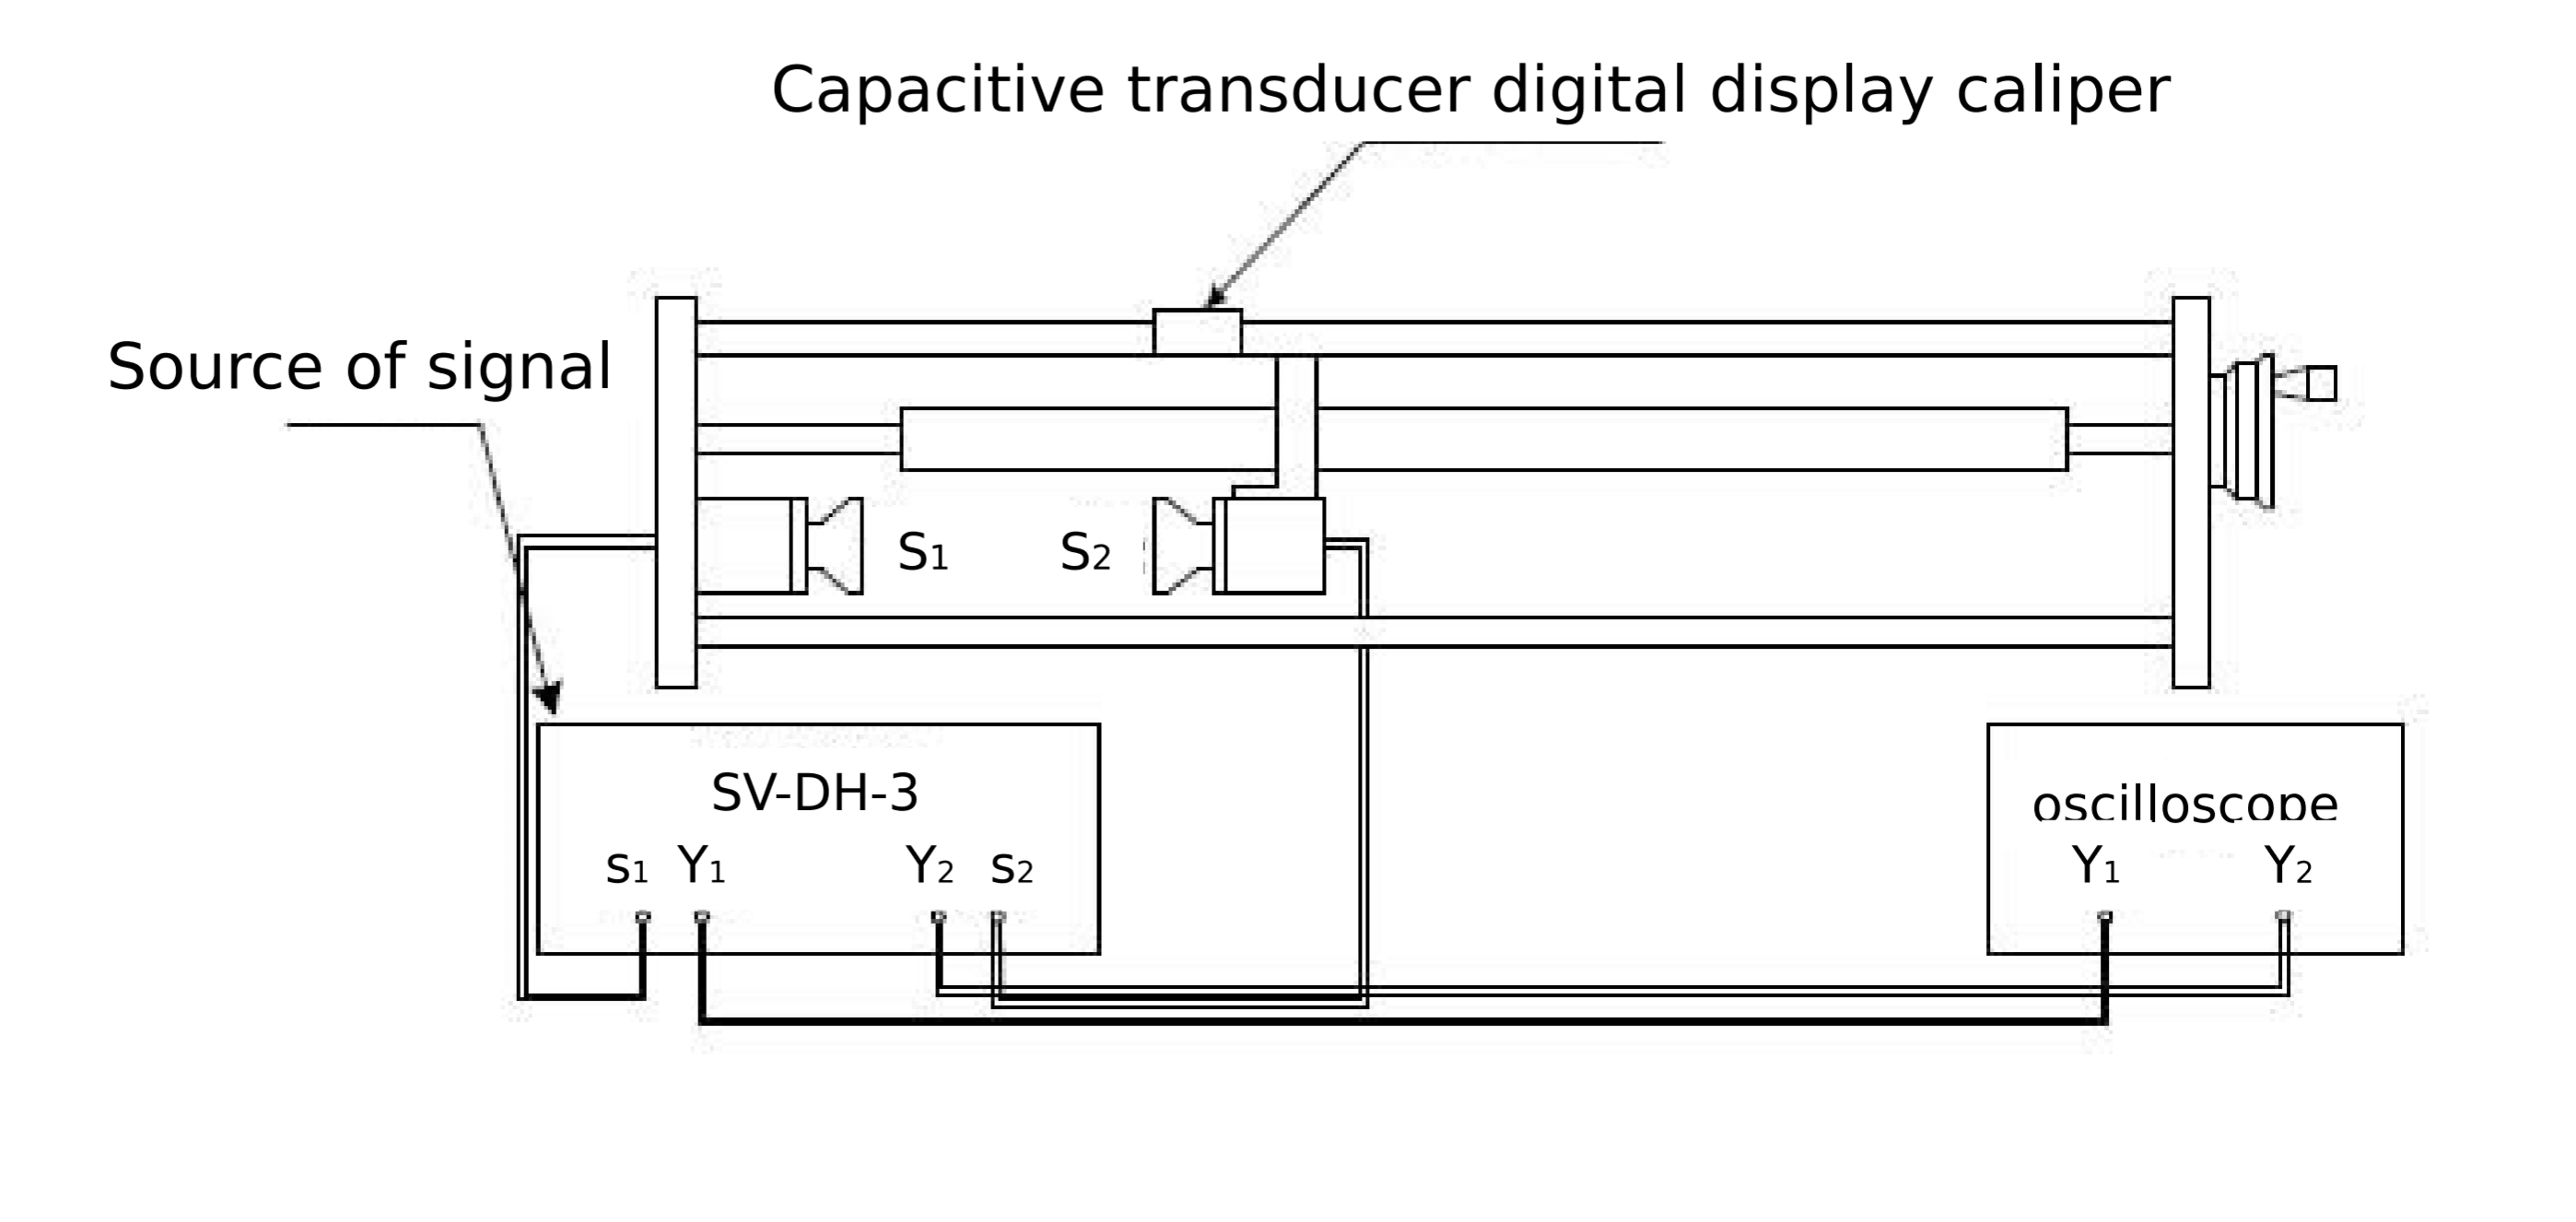
\includegraphics[width=0.8\textwidth]{Exset.png}
\caption{Experimental setup.}\label{Fig:Exset}
\end{figure}

\begin{table}[htbp]
\centering
\begin{tabular}{ccc}
  \hline
  Instrument & Measured quantities & Type-B uncertainties \\ \hline
  \multirow{2}{*}{Oscilloscope} & Frequency & 0.001\,kHz \\ & Time & 0.4\,$\mu$s \\ \hline
  Caliper & Distance & 0.001\,mm \\ \hline
  Thermometer & Temperature & 1\,$^{\circ}$C \\ \hline
\end{tabular}
\caption{Information of measurement instruments.}\label{Tab:Infof}
\end{table}


\section{Measurement Procedure}

\subsection*{Caution}
\begin{enumerate}
\item Make sure that $S_2$ moves in only one direction during each part of the experiment to avoid the backslash error.
\item When using the time-difference method, the initial distance between $S_1$ and $S_2$ should be greater than 10 cm. 
\item Prevent metal devices and callipers from contact with water when measuring the speed of sound in water.
\item Make sure that the distance between $S_1$ and $S_2$ is always greater than 1 cm.
\end{enumerate}

\subsection{Resonance Method}
\noindent In this part, you will adjust the distance between the two sources of signal and record the distance when the output voltage curves displayed on the screen reaches its maximum.

\begin{enumerate}
\item Set the initial distance between $S_1$ and $S_2$ at about 1 cm.
\item  Turn on the signal source and the oscilloscope. Then set the following options on the panel of the signal source
	\begin{enumerate}[(1)]
	\item Choose $Continuous$ wave for $Method$. 
	\item Adjust $Signal \,\,Strength$ until a 10 V peak voltage is observed on the oscilloscope. 
	\item Adjust $Signal \,\,Frequency$ between 34.5 and 40 kHz until the peak-to-peak voltage reaches its maximum. Record the frequency.
	\end{enumerate}
\item Increase $L$ gradually by moving $S_2$, and observe the output voltage of $S_2$ on the oscilloscope. Record the position of $S_2$ as $L_2$ when the output voltage reaches an maximum.
\item Repeat step 3 to record 12 values of $L_2$ and find $v$ by performing a linear fit to the data.
\end{enumerate}

\subsection{Phase-comparison Method}
\noindent In this part, you need to adjust the distance between the two sources of signal and record the distance when the Lissajous figures shown on the screen becomes a straight line.

\begin{enumerate}
\item Use Lissajous figures to observe the phase difference between the transmitted and the received signals. Move $S_2$ and record the position when the Lissajous figure becomes a straight line with the same slope.
\item Repeat step 1 to collect 12 sets of data and perform a linear fit to find $v$.
\end{enumerate}

\subsection{Time-difference Method in Liquid}
\noindent In this part, you will set the distance between the two source of signals and then measure the time spent to cover the distance by operating on the panel of the oscilloscope.

\begin{enumerate}
\item Change the medium to water.
\item Adjust the frequency to 100 Hz and the width to 500 $\mu$s.
\item Use the cursor function of the oscilloscope to measure the time and the distance between the the starting points of neighboring periods. Record 12 pairs of data and perform a linear fit to $v_\text{water}$.
\end{enumerate}



\section{Results}
\vspace{-6pt}
The measured frequency of the sound wave $f = 38.957\, [\text{kHz}] \pm 0.001\, [\text{kHz}]$.

The measured temperature $T = 23\,[^{\circ}\text{C}] \pm 1\, [^{\circ}\text{C}]$.
\vspace{-8pt}

\subsection{Resonance Method}

The measurement data of the resonance method is presented in Table \ref{Tab:ResMe}.

\begin{table}[htbp]
\centering
\begin{tabular}{cc}
\hline
\multicolumn{2}{c}{$L\, [\text{mm}] \pm 0.001\, [\text{mm}]$} \\
\hline
1 & 12.340 \\
2 & 16.886 \\
3 & 21.365 \\
4 & 25.927 \\
5 & 30.360 \\
6 & 34.940 \\
7 & 39.390 \\
8 & 43.984 \\
9 & 48.413 \\
10 & 52.986 \\
11 & 57.430 \\
12 & 61.991 \\
\hline
\end{tabular}
\caption{Measurement data for the resonance method.}\label{Tab:ResMe}
\end{table}

Plot $L$ vs. $n$ and apply linear fit using Origin, as is shown in Figure \ref{Fig:plot1}. The slope of the fit is $\alpha_1 = 4.511\,[\text{mm}] = 4.511 \times 10^{-3}\,[\text{m}]$ with uncertainty $u_{\alpha_1} = 0.006\,[\text{mm}] = 6 \times 10^{-6}\,[\text{m}]$. According to Eq.\ref{Eq:reasonance}, we obtain
\[ \lambda = 2 \alpha_1.\]
Combining this result with Eq.\ref{Eq:vlambdaf}, the speed of sound can be then calculated as
\begin{equation}\label{Eq:calofrea}
v = \lambda f = 2 \alpha_1 f = 2 \times 4.511 \times 10^{-3} \times 38.957 \times 10^3 = 351.5\,[\text{m/s}] \pm 0.5\,[\text{m/s}].
\end{equation}
with the relative uncertainty 0.13\,\%.

Theoretically, at 20\,$^{\circ}$C, the speed of sound in air is 344 [m/s]$^{[2]}$. The relative difference is then
\[\frac{|351.5 - 344|}{344} \times 100\% = 2.2\,\%.\]

\begin{figure}[htbp]
\centering
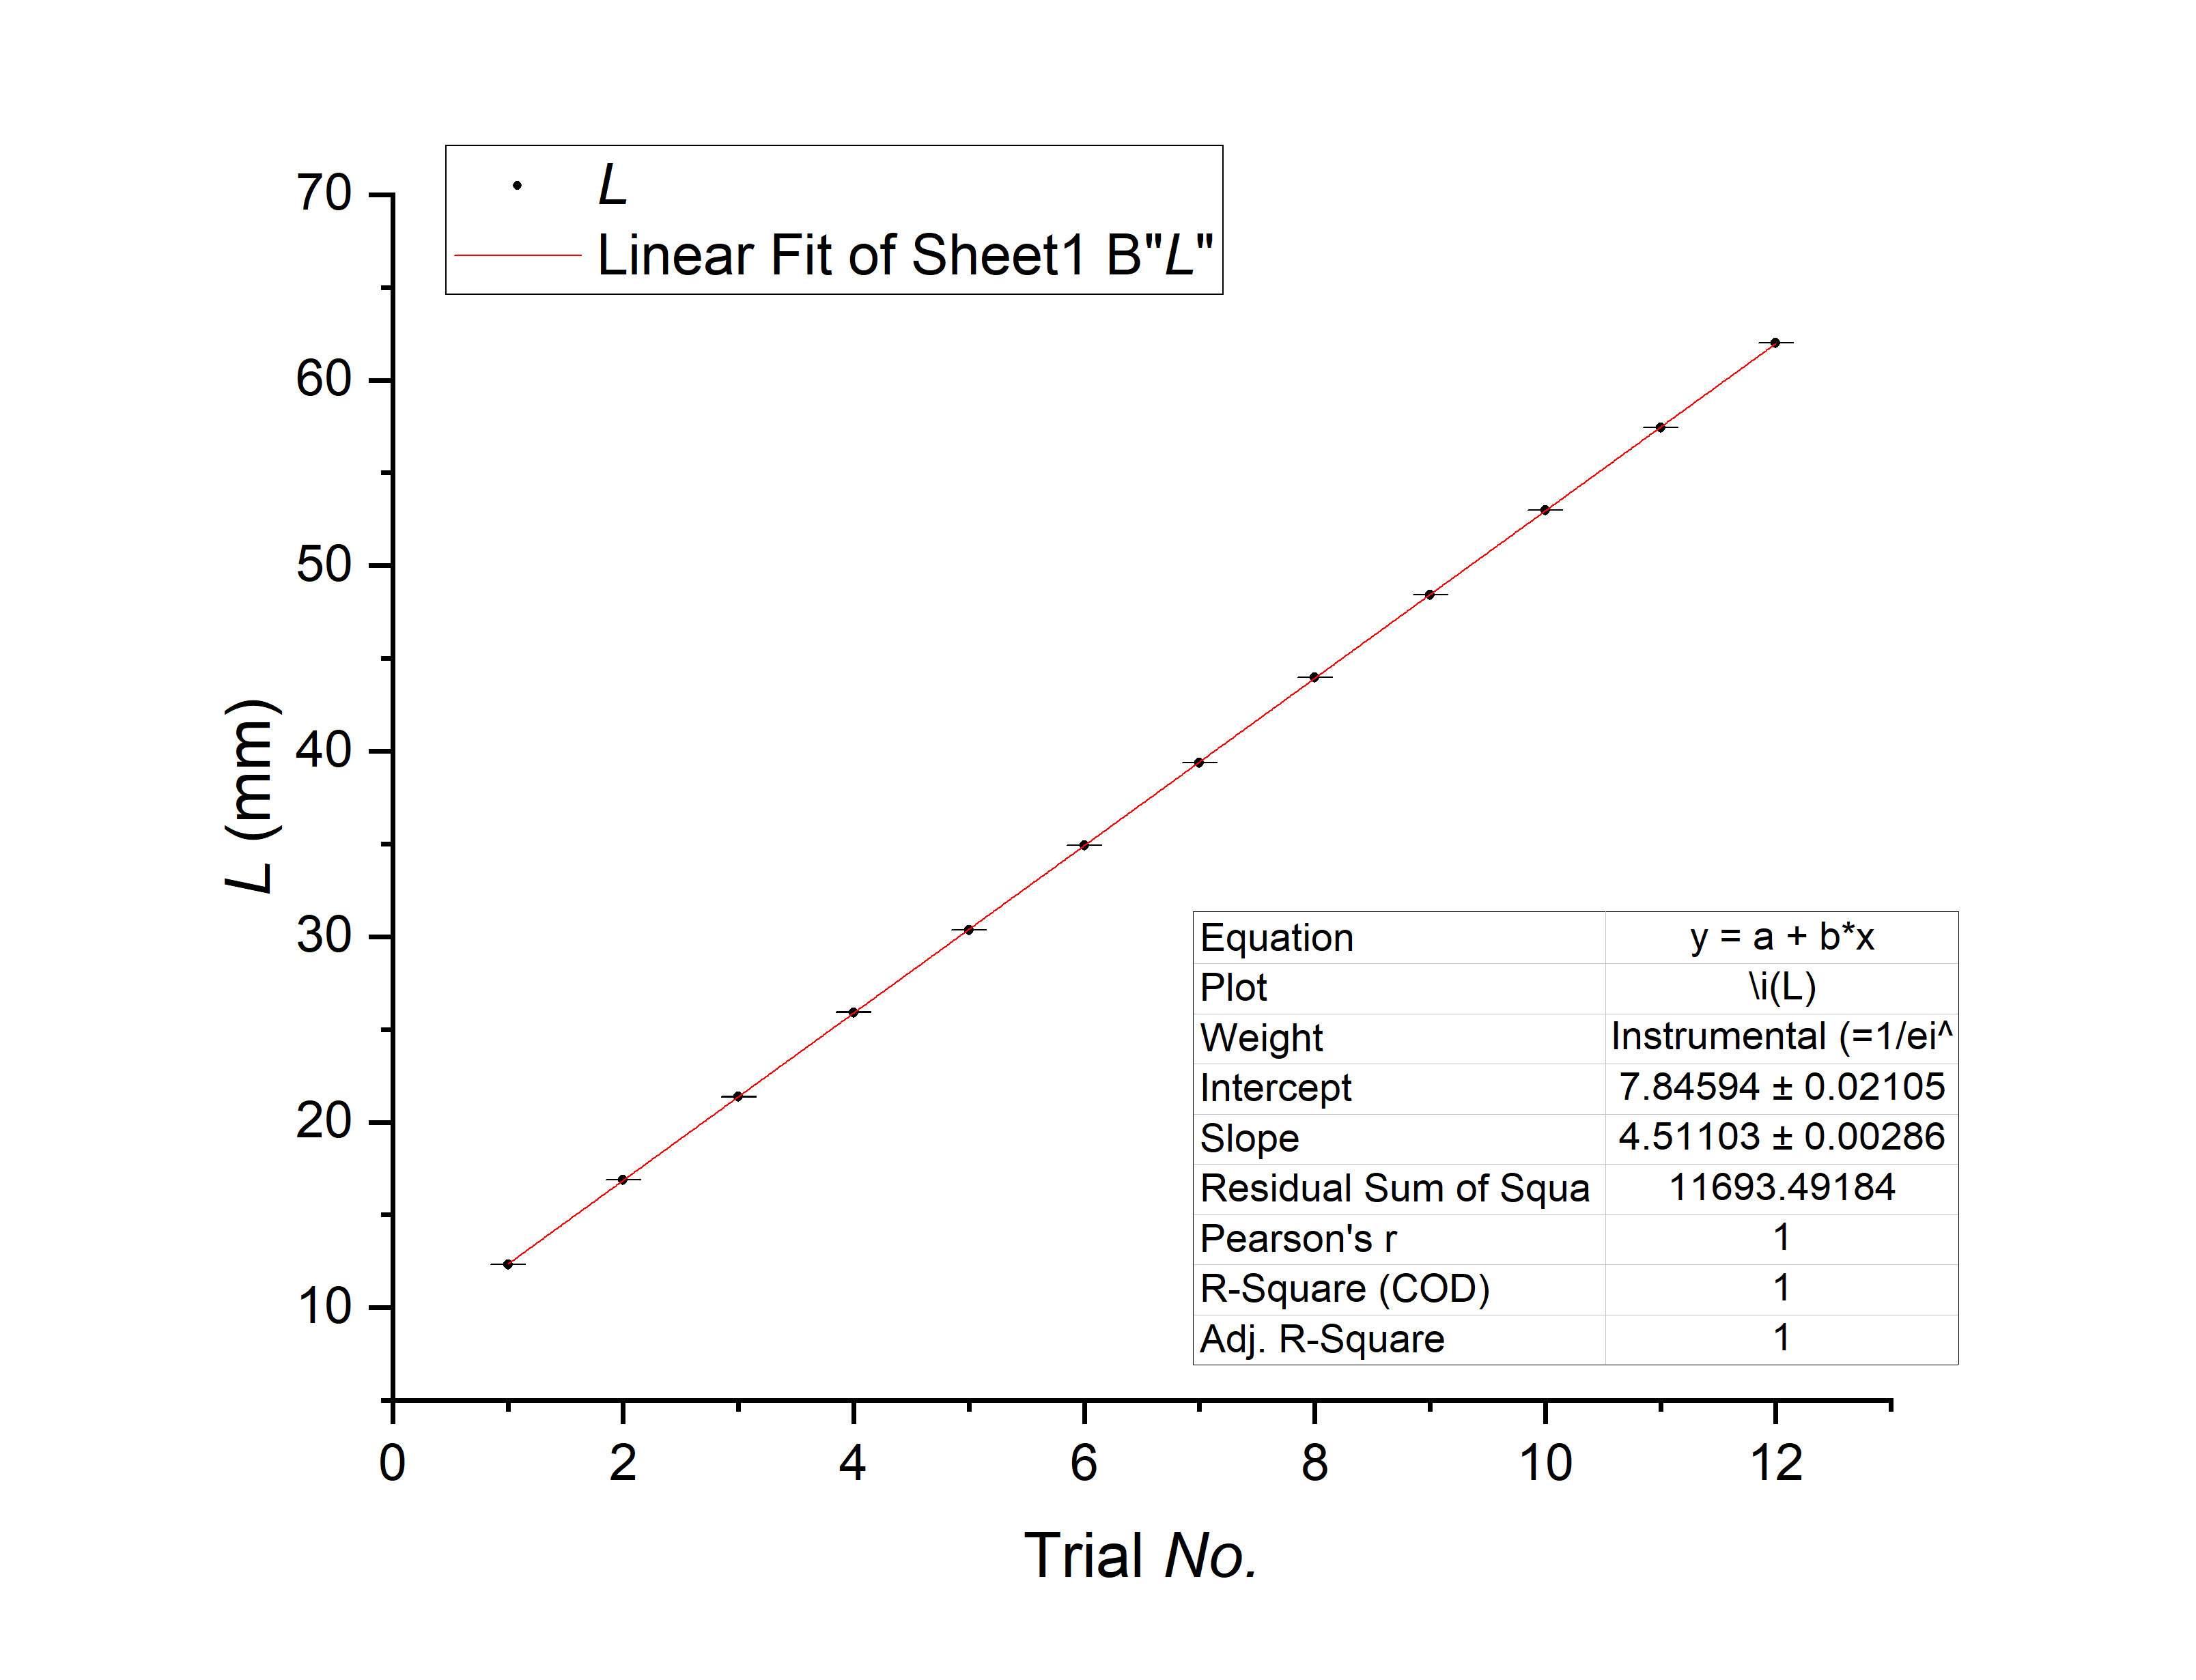
\includegraphics[width=0.8\textwidth]{plot1.png}
\caption{$L$ vs. $n$ for resonance method.}\label{Fig:plot1}
\end{figure}



\subsection{Phase-comparison Method}

The measurement data of the resonance method is presented in Table \ref{Tab:Phame}. 

\begin{table}[htbp]
\centering
\begin{tabular}{cc}
\hline
\multicolumn{2}{c}{$L\, [\text{mm}] \pm 0.001\, [\text{mm}]$} \\
\hline
1 & 21.330 \\
2 & 30.321 \\
3 & 39.323 \\
4 & 48.350 \\
5 & 57.318 \\
6 & 66.321 \\
7 & 75.298 \\
8 & 84.236 \\
9 & 93.229 \\
10 & 102.210 \\
11 & 111.133 \\
12 & 120.139 \\
\hline
\end{tabular}
\caption{Measurement data for the phase-comparison method.}\label{Tab:Phame}
\end{table}

Plot $L$ vs. $n$ and apply linear fit using Origin, as is shown in Figure \ref{Fig:plot2}. The slope of the fit is $\alpha_2 = 8.981\,[\text{mm}] = 8.981 \times 10^{-3}\,[\text{m}]$ with uncertainty $u_{\alpha_2} = 0.006\,[\text{mm}] = 6 \times 10^{-6}\,[\text{m}]$. According to Eq.\ref{Eq:phase}, we have
\[ \lambda = \alpha_2.\]
Combining this result with Eq.\ref{Eq:vlambdaf}, the speed of sound can be then calculated as
\begin{equation}\label{Eq:calofpha}
v = \lambda f = \alpha_2 f = 8.981 \times 10^{-3} \times 38.957 \times 10^3 = 349.9\,[\text{m/s}] \pm 0.2\,[\text{m/s}].
\end{equation}
with the relative uncertainty 0.07\,\%.

Theoretically, at 20\,$^{\circ}$C, the speed of sound in air is 344 [m/s]$^{[2]}$. The relative difference is then
\[\frac{|349.9 - 344|}{344} \times 100\% = 1.7\,\%.\]

\begin{figure}[htbp]
\centering
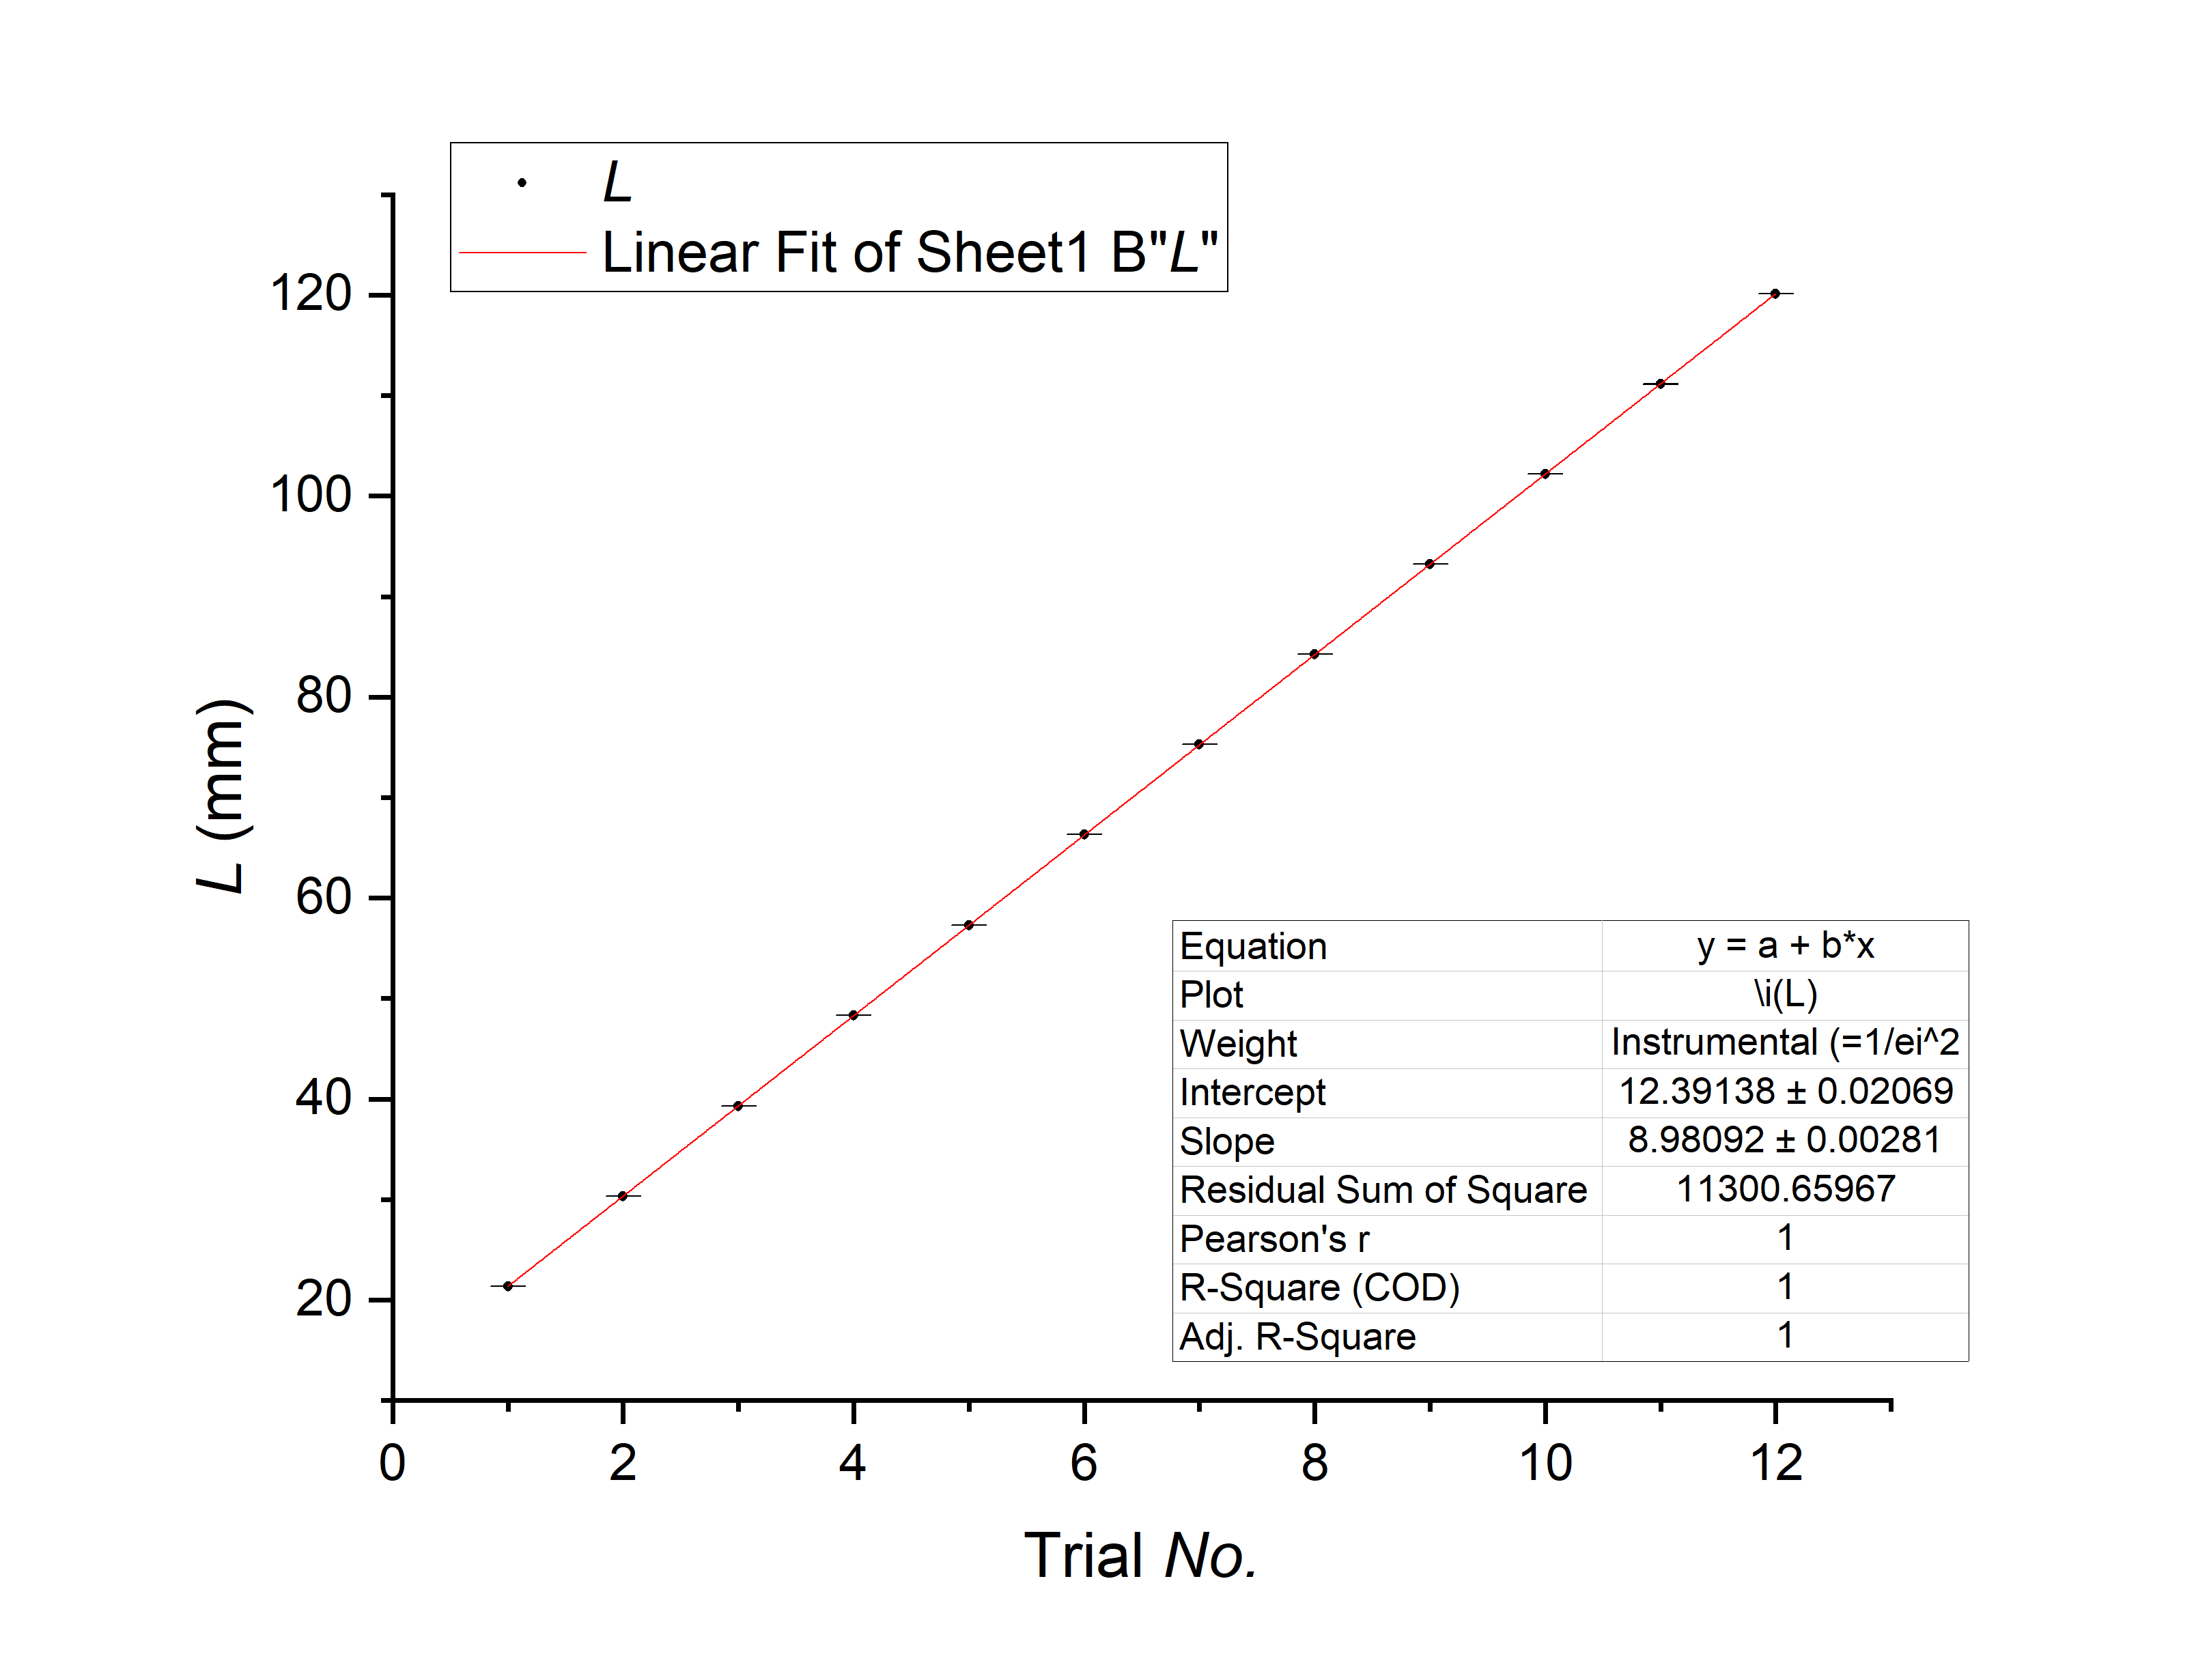
\includegraphics[width=0.8\textwidth]{plot2.png}
\caption{$L$ vs. $n$ for phase-comparison method.}\label{Fig:plot2}
\end{figure}



\subsection{Time-difference Method}

The measurement data of the resonance method is shown in Table \ref{Tab:Timdi}.

\begin{table}[htbp]
\centering
\begin{tabular}{ccc}
\hline
  & $L\, [\text{mm}] \pm 0.001\, [\text{mm}]$ & $t\,[\mu\text{s}] \pm 0.4\,[\mu\text{s}]$\\
\hline
1 & 110.000 & 81.6\\
2 & 120.000 & 87.6\\
3 & 130.000 & 94.4\\
4 & 140.000 & 100.8 \\
5 & 150.000 & 108.0\\
6 & 160.000 & 114.4\\
7 & 170.000 & 121.2\\
8 & 180.000 & 128.0\\
9 & 190.000 & 134.8\\
10 & 200.000 & 141.2\\
11 & 210.000 & 148.0\\
12 & 220.000 & 154.8\\
\hline
\end{tabular}
\caption{Measurement data for the time-difference method.}\label{Tab:Timdi}
\end{table}

Plot $t$ vs. $L$ and apply linear fit using Origin, as is shown in Figure \ref{Fig:plot3}. The slope of the fit is $\alpha_3 = 0.669\,[\mu\text{s/mm}] = 6.669 \times 10^{-4}\,[\text{s/m}]$ with uncertainty $u_{\alpha_3} = 0.004\,[\mu\text{s/mm}] = 4 \times 10^{-6}\,[\text{s/m}]$. According to Eq.\ref{Eq:vLt}, we have
\begin{equation}\label{Eq:caloftim}
v = \frac{1}{\alpha_3} = \frac{1}{6.669 \times 10^{-4}} = 1499\,[\text{m/s}] \pm 9\,[\text{m/s}].
\end{equation}
with the relative uncertainty 0.60\,\%.

Theoretically, at 20\,$^{\circ}$C, the speed of sound in water is 1482 [m/s]$^{[2]}$. The relative difference is then
\[\frac{|1499 - 1482|}{1499} \times 100\% = 1.13\,\%.\]

\begin{figure}[htbp]
\centering
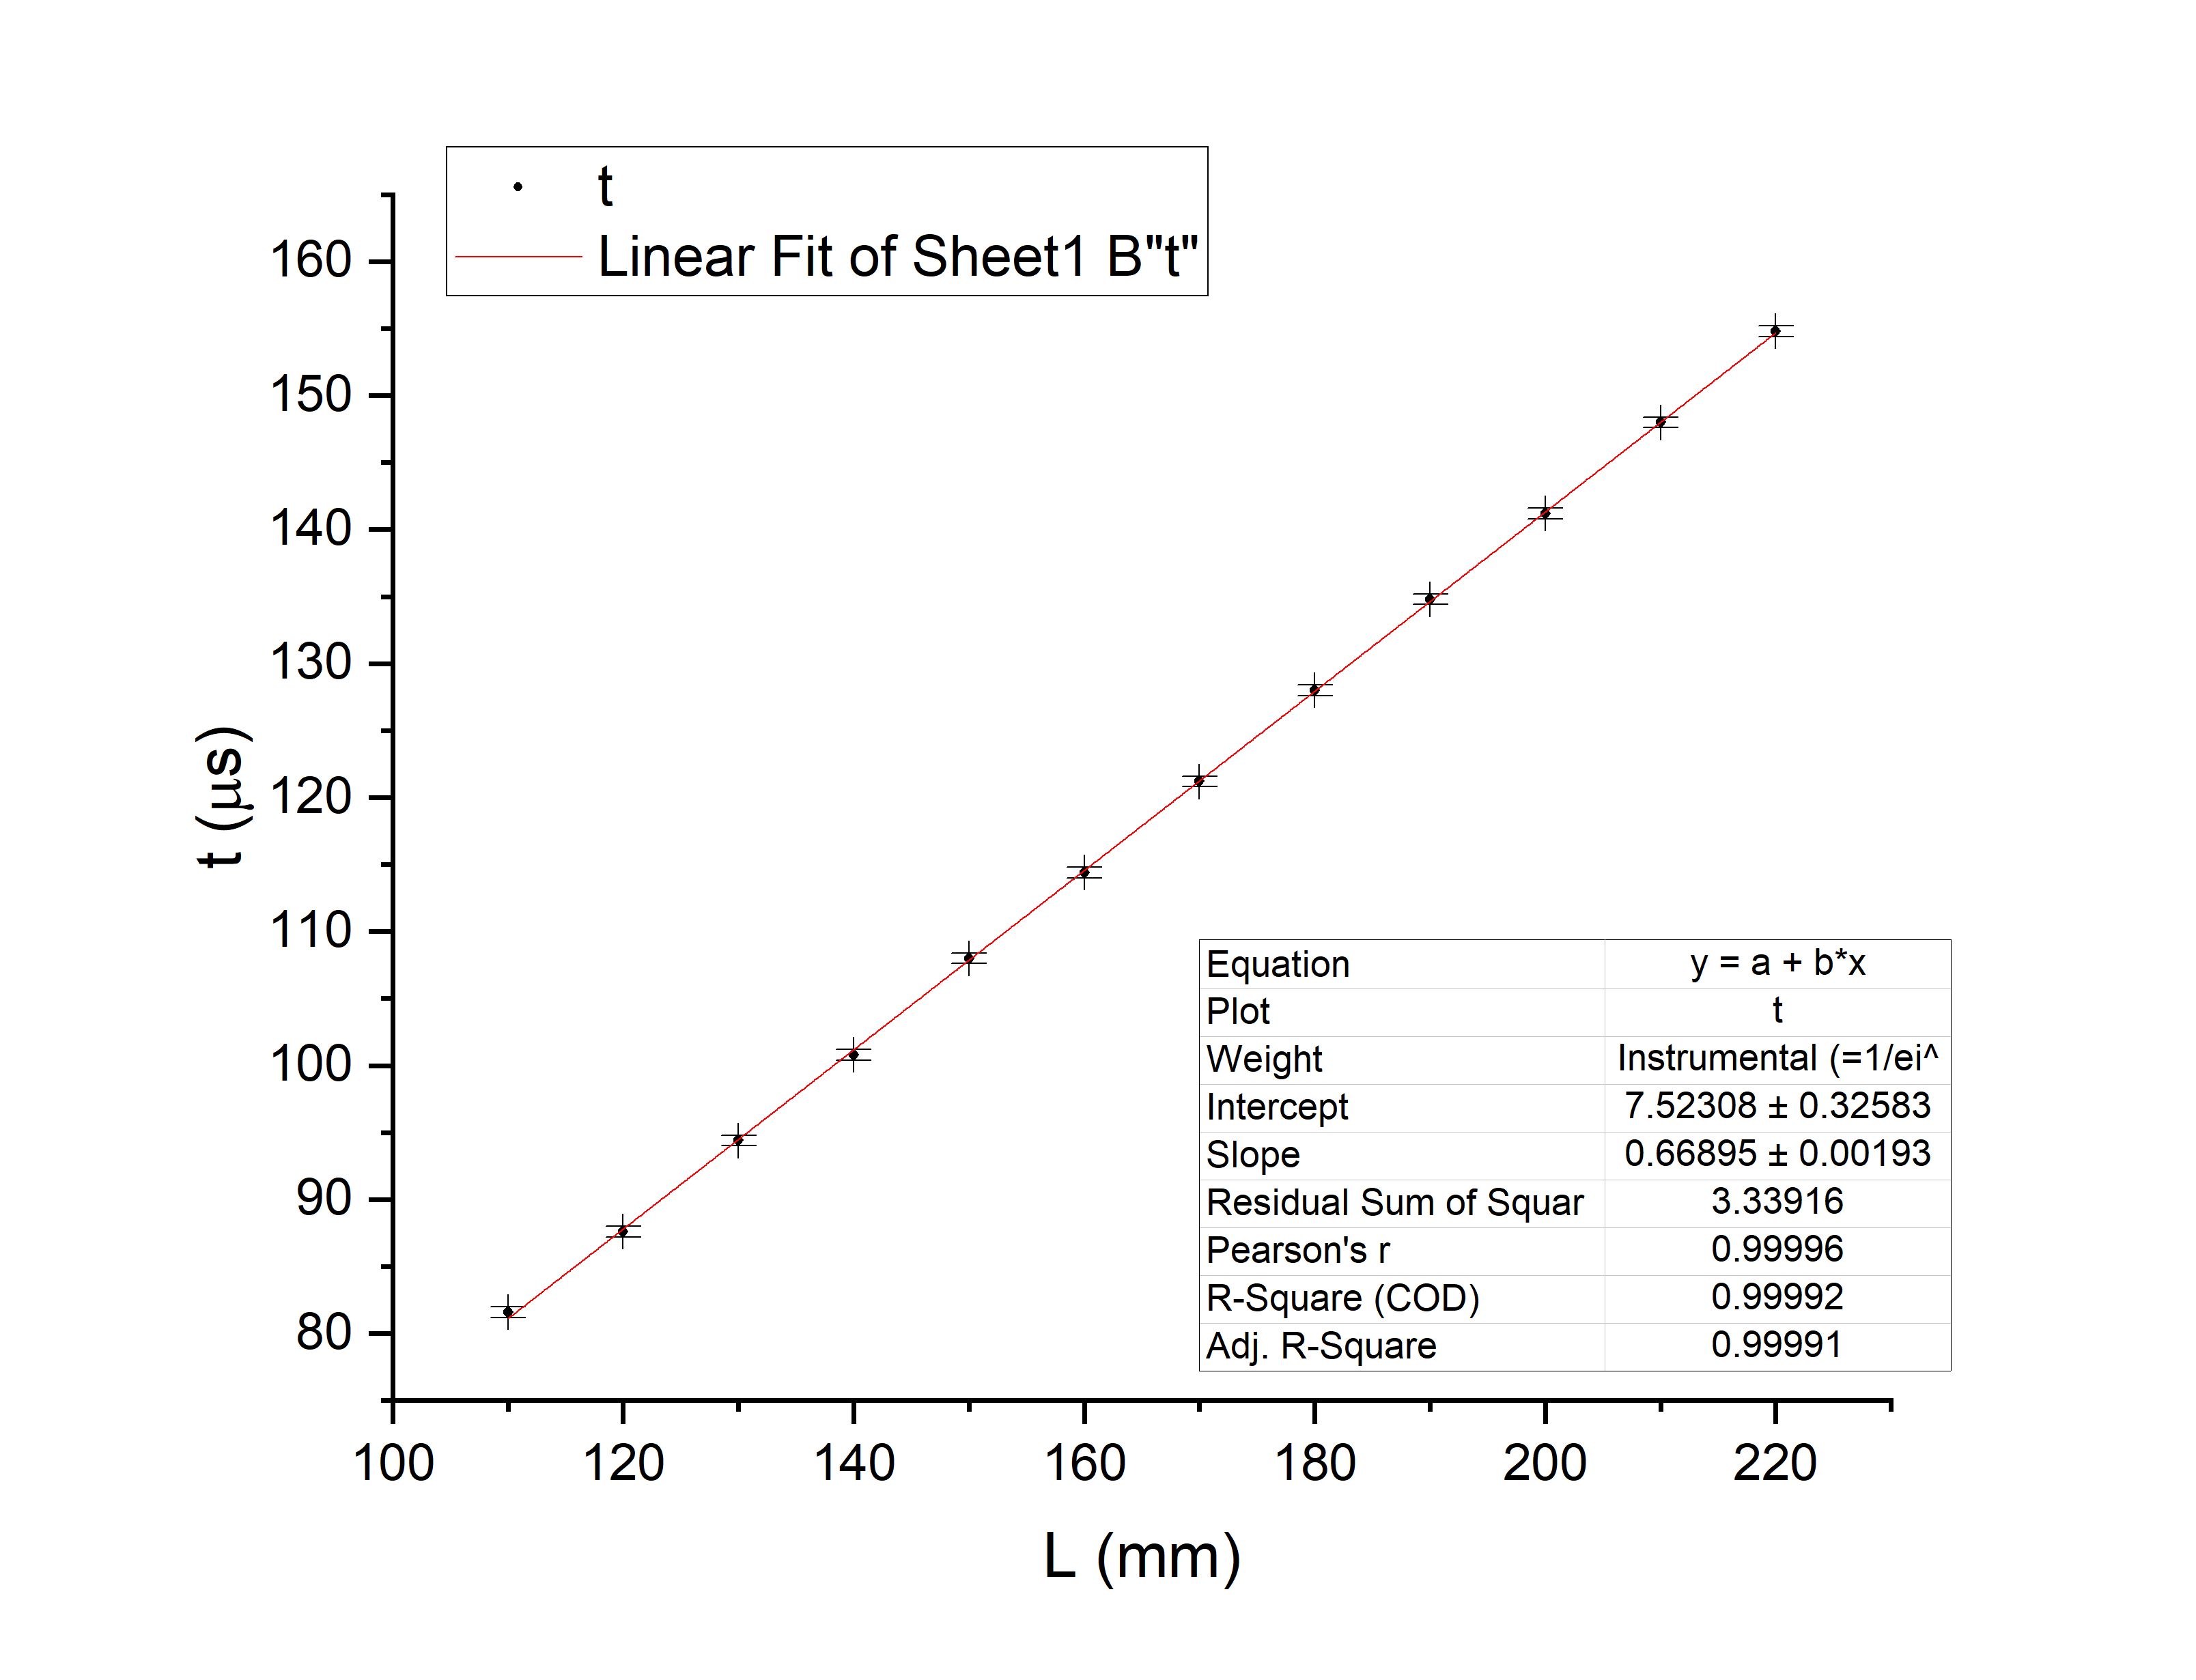
\includegraphics[width=0.8\textwidth]{plot3.png}
\caption{$L$ vs. $t$.}\label{Fig:plot3}
\end{figure}



\section{Conclusions and Discussion}
The results of the above analysis are summarized in Table \ref{Tab:result}.

\begin{table}[H]
\centering
\begin{tabular}{lcccc}
\toprule
& $v\,[\text{m/s}]$ & $u_{v,r}$ & $v_{\text{theory}}\,[\text{m/s}]^{[2]}$ & relative error\\
\midrule
Resonance(air) & 351.5 $\pm$ 0.5 & 0.13\,$\%$ & 344 & 2.2\,$\%$\\
Phase-comparison(air) & 349.9 $\pm$ 0.2 & 0.07\,$\%$ & 344 & 1.7\,$\%$\\
Time-difference (liquid) & 1499 $\pm$ 9 & 0.60\,$\%$ & 1482 & 1.13\,$\%$\\
\bottomrule
\end{tabular}
\caption{Experimental and theoretical results.}\label{Tab:result}
\end{table}

From Table \ref{Tab:result} it can be seen that the results conform to the theoretical and the errors are acceptable. Besides, as can be seen from Figure \ref{Fig:plot1}$\sim$\ref{Fig:plot3}, the R-square value r is close enough to 1 to show that the linear fit is rather fitting to the original data points. 

Still, some possible reasons of errors are listed in the following:
\begin{enumerate}
\item The knob for adjusting the distance is loose, which may rotate after we have adjusted the distance and thus cause error.
\item The theoretical speed of sound shown in Table \ref{Tab:result} is at the temperature of 20$^{\circ}$C. In our experiment, however, the temperature is measured to be $23\,[^{\circ}\text{C}] \pm 1\, [^{\circ}\text{C}]$, which is higher than 20$^{\circ}$C. The temperature can result in the difference between theoretical values and the experimental results (This is also the reason why we need to measure temperature in our experiment).
\item Also, the theoretical speed of sound in water shown is in the conditions of pure water. The water used in our experiment is not pure, which can lead to inaccuracy.
\item In the phase-comparison method, we can't make sure that the Lissajous figures become exactly straight lines every time. However, we have already optimize this method by choosing the ``straight line'' Lissajous figures as reference. It is much easier and can cause less error to judge that the figure forms a straight line than to judge that the figure becomes an ellipse of the same shape and size (and that is the reason why we use the ``straight line'' Lissajous figures as reference).
\item Similarly, in the resonance method, we need to arrive at the maximum of the output voltage showed on the screen, but we can't make sure that we make it exactly at the maximum point. (This is related to the reason why we use the resonance frequency. At resonance frequency, the output voltage will be greater and ``steeper'', which will thus make it more easier and cause less error to judge whether the output voltage has reached its maximum. Otherwise, the error may become larger.)
\end{enumerate}

Note that there are other operations specified in our experiment which can help reduce the error. For example, in the time-difference method, the $L$ is set to be greater than 100\,[mm], which ensures that a certain time interval is needed to cover $L$ so that the time interval measured is not too small and thus the relative error of the measurement of the time interval is relatively small.

We can also see from Table \ref{Tab:result} that the resonance method gives the result of medium uncertainty and largest relative error; the phase-comparison method gives the result of least uncertainty and medium relative error; the time-difference method gives the result of greatest uncertainty but with least relative error. With the above analysis of the factors that contribute to error and uncertainty, we can somehow interpret such a comparison of the three methods. The relatively greater uncertainty of time measurement results in the greatest uncertainty of the time-difference method; the maximum output voltage is harder to be judged, which leads to the greatest relative error of the resonance method.

\vspace{8pt}
In my opinion, the ideas below may help improve the experiment:
\begin{enumerate}
\item Wash the container of water. Clean and purify the water in it. 
\item Keep the room temperature constant at 20\,$^{\circ}$.
\item Use devices of higher resolution and sensitivity to make it easier for us to judge whether the output voltage reaches its maximum and whether the Lissajous figures forms a straight line and thus reduce the corresponding error.
\end{enumerate}



\section{Reference}

\noindent [1] Qin Tian, et al. editor.``VP141 Exercise 4: Measurement of the Speed of Sound''.

\noindent [2] Young and Freedman. \textit{University Physics with Modern Physics}. pp. 516, Table 16.1.

\newpage



\appendix

\section{Uncertainty Analysis}

\subsection{Uncertainty of Resonance Method}
Apply the uncertainty propagation formula to Eq.\ref{Eq:calofrea},
\[u_v = \sqrt{{(\frac{\partial v}{\partial \alpha_1})}^2u_{\alpha_1}^2 + {(\frac{\partial v}{\partial f})}^2u_f^2} = \sqrt{4 f^2 u_{\alpha_1}^2 + 4 {\alpha_1}^2 u_f^2} = 0.4676 = 0.5 \,[\text{m/s}],\]
and the relative uncertainty is
\[u_{r,v} = \frac{u_v}{v}\times 100\% = \frac{0.4676}{351.5}\times 100\% = 0.13\%.\]

\subsection{Uncertainty of Phase-comparison Method}
Apply the uncertainty propagation formula to Eq.\ref{Eq:calofpha},
\[u_v = \sqrt{{(\frac{\partial v}{\partial \alpha_2})}^2u_{\alpha_2}^2 + {(\frac{\partial v}{\partial f})}^2u_f^2} = \sqrt{ f^2 u_{\alpha_2}^2 + {\alpha_2}^2 u_f^2} = 0.2339 = 0.2 \,[\text{m/s}],\]
and the relative uncertainty is
\[u_{r_v} = \frac{u_v}{v}\times 100\% = \frac{0.2339}{349.9}\times 100\% = 0.07\%.\]

\subsection{Uncertainty of Time-difference Method}
Apply the uncertainty propagation formula to Eq.\ref{Eq:caloftim},
\[u_v = \sqrt{{(\text{--}\,\frac{1}{{\alpha_3}^2})}^2 u_{\alpha_3}^2} = \frac{u_{\alpha_3}}{{\alpha_3}^2} =  8.994 = 9 \,[\text{m/s}],\]
and the relative uncertainty is
\[u_{r_v} = \frac{u_v}{v}\times 100\% = \frac{8.994}{1499}\times 100\% = 0.60\%.\]



\section{Data Sheet}

See the last two pages.

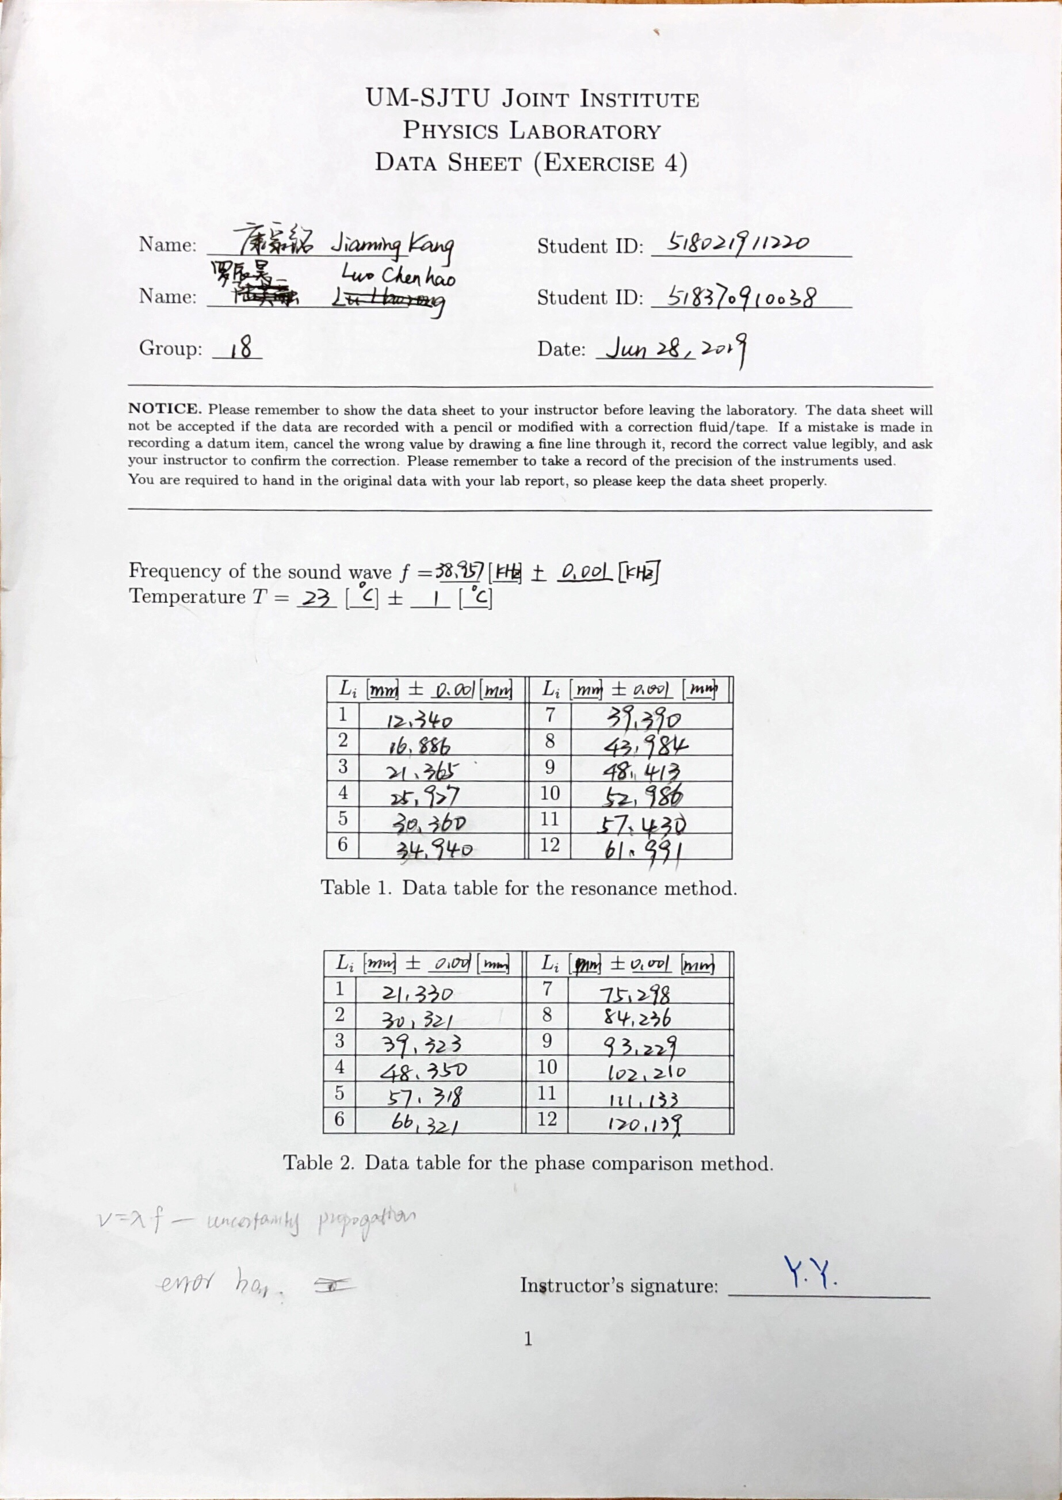
\includepdf[pages=-]{lab4_datasheet.pdf}



\end{document}
